\section{Practical 1 - Git, Bash, GPIO}
\label{sec:Prac1}
\subsection{Overview}
This practical sets out to familiarise you with the Pi and complete a simple programming task. If you have not yet done so, complete Prac 0. Ensure that you can SSH into the pi, as all the tasks for this prac require it.

\subsection{Pre-prac Requirements}
This section covers what you will need to know before starting the practical.
\begin{itemize}
    \item Have your Raspberry Pi Set up as per the requirements of Prac 0.
\end{itemize}

\subsection{Outcomes}
You will learn about the following aspects:
\begin{itemize}
    \item SSH
    \item VNC
    \item Git
    \item Bash
    \item Basic GPIO usage
\end{itemize}

\subsection{Deliverables}
At the end of this practical, you must:
\begin{itemize}
    \item Demonstrate your working implementation to a tutor
    \item Submit your screenshots from the Terminal task to Vula in a pdf document
    \item Submit your Python code (along with the .git folder) to Vula
\end{itemize}

\subsection{Hardware Required}
\begin{itemize}
    \item Raspberry Pi
    \item SD Card
    \item Ethernet Cable
    \item 2 x pushbuttons
    \item 3 x LEDs
    \item 3 x Resistors
    \item A breadboard
    \item Jumper wires
\end{itemize}

\subsection{Walkthrough}
\subsection{Terminal}
\label{sec:Prac1:Terminal}
While there are many Graphic User Interfaces (GUI) available for various distributions of Linux including Raspbian, it is often necessary to operate an embedded system without a GUI given the limited processing and memory resources of the device.  Consequently it is important to learn to use Linux through the command line shell, a very common shell on many linux systems is known as Bash.  There is a lot to learn and a being comfortable with the command line will help you greatly in working with embedded systems,  The following will introduce the basics to you but if you have never used a Linux command line before we suggest you go through the following exercise in your own time  and if you are interested or have the time this 4hr online lesson will give you a very good grounding: https://swcarpentry.github.io/shell-novice/

Start by SSH'ing into your Pi and create a folder called \textless your\_student\_number\textgreater.\\
Run the following commands, and take a screenshot after each command:
\begin{itemize}
    \item ls (must show the folder you just created)
    \item ifconfig (etho0 must be visible)
    \item lscpu (number of cores must be visible)
\end{itemize}
Your result should look something like this:
\begin{figure}[H]
\centering
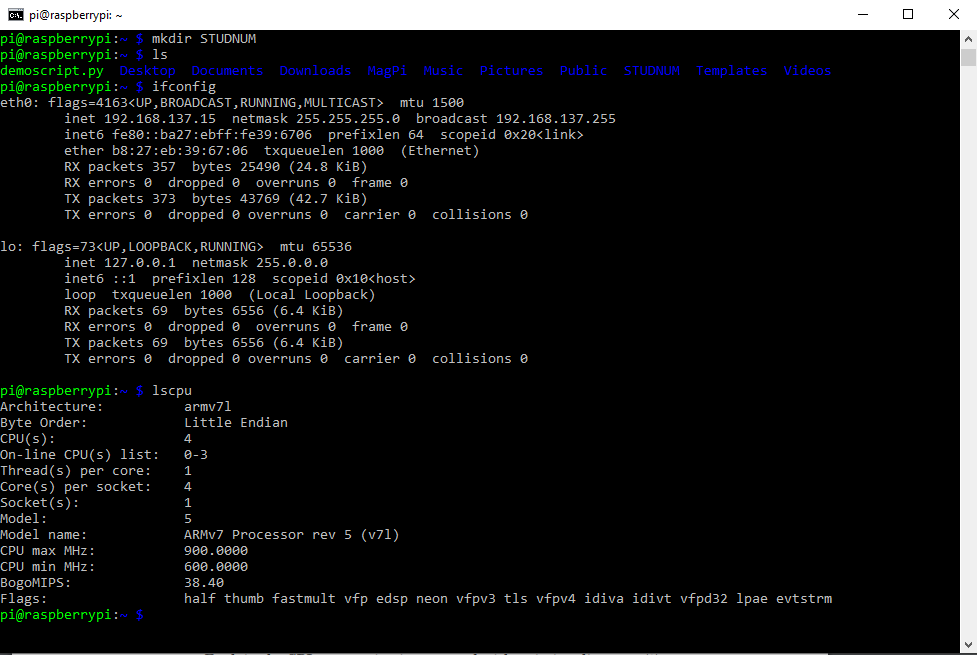
\includegraphics[width=0.6\columnwidth]{Figures/CMDOutput}
\caption{Example output after running the above commands}
\label{fig:CMDOutput}
\end{figure}



\subsubsection{Programming Task 1}
In this task you will develop a simple 3-bit binary counter, the values of which will be placed on LEDs connected to the Pi. The value on the counter should change every 1 second, and should count up from 0 to 7, and then go back to 0.
Be sure to use git to keep track of changes to your code. For instructions on using Git, take a look at Section \ref{sec:Git}.
\begin{itemize}
    \item Start by connecting to your Pi through VNC (see Section \ref{app:Services-VNC})
    \item Connect 3 LEDs and 2 Push buttons to the GPIO pins of the Pi following this circuit
    \item Read the Python Tips and tricks in Section \ref{app:Python} to gain understanding of the commands and why they are used.
    \item Open Geany (or another text editor of your choice), and create a copy of the template given to you in the appendix.
    \item Test the GPIO pins of the RPi by turning LEDs on and off without any iteration logic. You can use \textit{time.sleep()} from the time library to wait between turning them on and off.
    \item Write your logic (Hint: Look at \textit{itertools.product} to generate a list of binary values.)
    \item push your working code to github
    \item demonstrated operation to tutor and get signed off
\end{itemize}

\subsection{Programming Task 2}
Using the code above, add some buttons to increment, decrement and reset the values on the LEDs. Make sure to use interrupts, as explained in Section \ref{app:Python}. Demonstrate this functionality to a tutor.


% \subsection{Bonus Tasks}
% These tasks are not for marks, but instead are given to allow you to learn more about the Raspberry Pi and networking. 
% \begin{itemize}
%     \item Configure the Raspberry Pi as a WiFi hotspot, and connect your phone/another Pi to it and ping it.
%     \item Use threading in your prac to trigger the counter update (see Section \ref{app:Python})
%     \item Count up and then down, rather than just counting up and resetting to zero
%     \item Connect to Eduroam using wpa\_supplicant configuration
%     \item Create a two node cluster between two RPis with one master RPi telling the other slave RPi what to run. \textbf{TODO: Provide the students with commands to do this with explanations} 
% \end{itemize}
